\documentclass[titlepage]{article}

\usepackage[margin=2cm]{geometry}

\usepackage{amsmath}
\usepackage{amsfonts}
%\usepackage{braket}
\usepackage{tabularx}
\usepackage{amsthm}
\usepackage[braket, qm]{qcircuit}
%\usepackage[bookmarks = true, pdfpagemode = None, pdfstartview = FitH, colorlinks = true, urlcolor = blue]{hyperref}
\usepackage{listings}
\usepackage{caption}
\usepackage{subcaption}
\usepackage{graphicx}
\usepackage{algorithm}
\usepackage{placeins}
%\usepackage{algorithmic}
\usepackage[noend]{algpseudocode}
\makeatletter
% Reinsert missing \algbackskip
\def\algbackskip{\hskip-\ALG@thistlm}
\makeatother
\renewcommand{\arraystretch}{1.5}

\theoremstyle{definition}
\newtheorem{definition}{Definition}[section]

\theoremstyle{problem}
\newtheorem{problem}{Problem}[section]

\theoremstyle{lemma}
\newtheorem{lemma}{Lemma}[section]

\usepackage{pdfpages}
\usepackage{epspdfconversion}
\usepackage{xcolor,colortbl}

\title{Efficient Near-Optimal Clifford + T Gate Synthesis}
\author{Luke Heyfron, and Earl T. Campbell}
\date{October 2017}

\begin{document}
	\maketitle
	\begin{abstract}

	\end{abstract}
	
	\section{Introduction}
		% Motivation:
		% 	- Use an example of optimal run time on a known circuit to motivate development of efficient heuristics.
		%	- (T gates are expensive)
		%	- Problem definition: exact multi-qubit non-unitary Clifford + T synthesis problem
		%	- Motivate problem: exact optimal single qubit synthesis essentially solved; multi-qubit believed to be hard; by relaxing problem to allow for non-unitary processes such as ancillas and measurements we have developed an efficient Clifford + T near optimal gate synthesis protocol by borrowing from techniques for symmetric tensor contracting on GF(2).
		%	- Paper overview: Section 1 intoduction and motivation; section 2, 3 description of the high and low levels respectively of the T gate optimization protocol main result of this paper. Section 4 discuss results for T counts numerical resultant from this algorithm and compared to others. Section 5 Discuessions and conclusions for future work.
		\iffalse
		T gates are expensive toric code transversal gates high threshold Clifford operations.		
		exact optimal single qubit synthesis essentially solved; multi-qubit believed to be hard; by relaxing problem to allow for non-unitary processes such as ancillas and measurements we have developed an efficient Clifford + T near optimal gate synthesis protocol by borrowing from techniques for symmetric tensor contracting on GF(2).
		exact multi-qubit non-unitary Clifford + T synthesis problem given an n qubit input circuit U that can be synthesized exactly using gate from Clifford + T gate set, find a circuit U' on n+h qubits that implements U on the first n qubits and the final h qubits are not entangled with the first n using minimal number of T gates.
		We have developed an efficient T-gate optimization protocol that finds nearly optimal solutions to the above problem.
		An overview of the paper is as follows. Section 1 introduction and motivation; section 2, 3 description of the high and low levels respectively of the T gate optimization protocol main result of this paper. Section 4 discuss results for T counts numerical resultant from this algorithm and compared to others. Section 5 Discussions and conclusions for future work.
		\fi
		
	\FloatBarrier		
		
	\section{Workflow Overview}
		\label{sec_methods}
		% ------- VERSION 1 ------
		% Workflow  description
		\iffalse
		We now describe the high level workflow of our T gate optimization protocol. The Clifford + T gate set is desirable as it forms a universal gate set, however the optimizer acts directly on diagonal circuits composed of CNOT and T gates only, so the first step of the protocol is to extract a circuit of the desired gate set from an arbitrary circuit from the Clifford + T gate set. This is done using the Hadamard gadget depicted in figure \ref{fig_hadamards}, which allows us to replace internal Hadamards with an ancilla prepared in the $\ket{+}$ state, upon which we post-select the $\ket{+}$ outcome at the end of execution. It can be shown that any CNOT+T circuit $W$ can be decomposed as $W=U_fV$ where $V$ is composed of CNOT gates only with zero T count, and $U_f$ acts on each $n$-qubit computational basis state $\mathbf{x}\in \mathbb{Z}_2^n$ as
		\begin{equation}
			U_f\ket{\mathbf{x}} = \omega^{f(\mathbf{x})}\ket{\mathbf{x}},
		\end{equation}
		where $\omega = e^{i\frac{\pi}{4}}$ and $f:\mathbb{Z}_2^n \mapsto \mathbb{Z}_8$ is known as the \emph{phase function}.

		The phase function can be decomposed into the form,
		\begin{equation}
		f(x) = \sum_{\alpha=1}^{n}l_{\alpha}x_\alpha + 2\sum_{\alpha<\beta}^{n} q_{\alpha,\beta}x_\alpha x_\beta + 4\sum_{\alpha,\beta,\gamma}^{n}c_{\alpha<\beta<\gamma}x_\alpha x_\beta x_\gamma \pmod{8}
		\end{equation}
		which we refer to as the \emph{weighted polynomial}.
		
		We define the signature tensor $S$ of a unitary $U_f$ to be the parity of the weighted polynomial coefficients, i.e. $S_{\alpha,\alpha,\alpha} = l_{\alpha} \pmod{2}$; $S_{\alpha,\beta,\beta} = S_{\alpha,\alpha,\beta} = q_{\alpha,\beta} \pmod{2}$ etc.
		It can be shown that the signature tensor is unique for each unitary in $\mathcal{D}_3$ up to Clifford equivalence, hence is a useful way to characterize such unitaries. %The signature tensor is an object conserved between pairs of Clifford equivalent CNOT+T circuits.
		
		% ------- VERSION 2 --------
			
		The core of our protocol is an algorithm for optimizing the T count of CNOT+T circuits. In order for the protocol to accept Clifford+T circuits we take an approach similar to 
		\fi
		
%\subsection{Workflow Overview}
\label{ssec_workflow}

The high level workflow of the protocol begins by converting an $n$ qubit input Clifford + $T$ circuit, $C_{\text{in}}$, (fig. \ref{fig_overview}.1) to a CNOT + $T$ circuit plus additional operations that are all Clifford (fig. \ref{fig_overview}.2). The purpose of this is to isolate the non-Clifford behaviour within a subcircuit that has properties required for our optimization framework (see section \ref{ssec_diag}). The main obstacle to this conversion process is the presence of Hadamard gates in the original circuit. External Hadamards, found at the beginning and end of the circuit, can be left in place. In order to remove internal Hadamards we use an approach similar to that of \cite{1_Montanaro_2017}, \cite{2_Bremner_2010} where a unitary Hadamard gate is replaced with a Hadamard gadget that involves only CNOT + T gates as well as preparation of ancillas in the $\ket{+}$ state and measurement in the Pauli-$X$ basis (see figure \ref{fig_hadamards}). In doing so we are trading internal Hadamards for external Hadamards and space-like overhead.

Once the Hadamards are removed, we decompose the CNOT + T circuit into two partitions such that one part consists of CNOT gates only and the other is diagonal in the computational basis (fig. \ref{fig_overview}.3).
We then extract the \emph{signature tensor} of the diagonal CNOT + T circuit, which is an object that uniquely characterizes the unitary $U_f$ up to a Clifford factor. 

The core layer of the algorithm, \emph{T-optimiser}, takes as input the signature tensor of the diagonal CNOT + T circuit and outputs a \emph{gate synthesis matrix}, $A$, which represents a particular circuit decomposition for the input unitary. The number of columns of $A$ is equal to the $T$ count of its corresponding circuit, so \emph{T-optimiser} ideally outputs a gate synthesis matrix with minimal column number. It is believed that finding optimal solutions for this problem is NP-hard \cite{3_Amy_2016}, so we must use efficient heuristics that yield near-minimal column number.

The output $A$ matrix is mapped to a circuit of the same form as $U_f$, with which the original $U_f$ circuit is replaced. The result is an output circuit that implements the full Clifford + $T$ input circuit on the first $n$ qubits and has near optimal $T$ count.

\begin{figure}[h!]		
			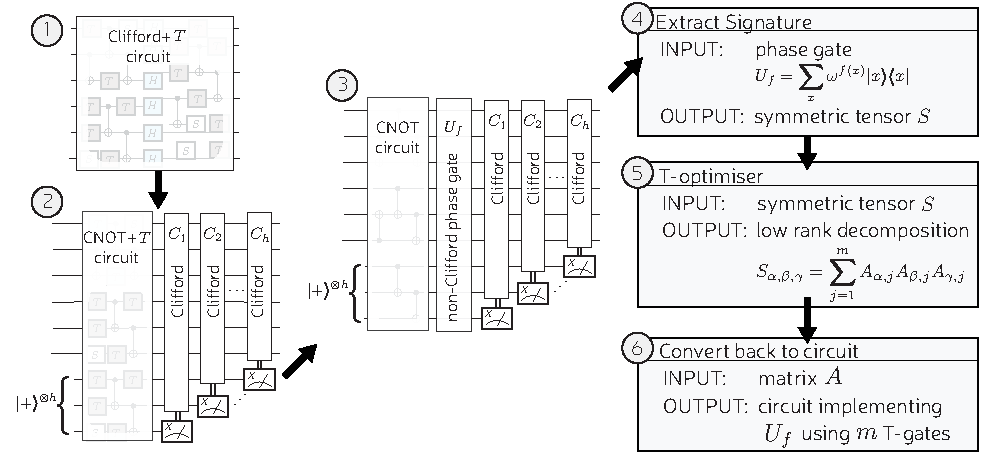
\includegraphics{Overview3}
			\caption{The high level workflow of the T gate optimization protocol is shown. A Clifford + T circuit is converted to the CNOT+T gate set by introducing ancillas and performing classically controlled Clifford gates. A non-Clifford phase gate is extracted, which maps to a signature tensor upon which the core optimization algorithm is performed. The optimized symmetric tensor decomposition is then converted back into a circuit of the form in panel 2) yielding an implementation of the original Clifford + T circuit with reduced T count. }
			\label{fig_overview}
		\end{figure}

\begin{figure}[h]
			\[
				\Qcircuit @C=1em @R=1em {
					\lstick{\ket{\psi}} & \gate{H} &  \rstick{H\ket{\psi}}\qw & &\push{\rule{2em}{0em}=\rule{2em}{0em}} &  \lstick{\ket{\psi}} & \ctrl{1} & \qw & \qswap & \qw & \gate{X} & \rstick{H\ket{\psi}}\qw \\
					& & & & & \lstick{\ket{+}} &  \ctrl{-1} & \qw & \qswap \qwx & \qw & \meter \cwx & \dstick{X}
				}
			\]
			\caption{Internal Hadamards are removed by replacing each one according to this circuit identity. The Hadamards on the left-hand circuit are now external and act on an ancilla, therefore they no longer obstruct the \emph{T-optimiser} algorithms.}
			\label{fig_hadamards}
		\end{figure}

\FloatBarrier
\section{Diagonal CNOT+T Framework}
\label{ssec_diag}

This section describes how we map the gate synthesis problem from the quantum circuit picture to an abstract mathematical picture involving binary tensors. We proceed by borrowing the observation from \cite{5_Amy_2013},\cite{6_Amy_2013} that the action of any $n$-qubit diagonal CNOT + $T$ unitary $U_f$ on a computational basis state $\ket{\mathbf{x}}$ is given by
\begin{equation}
U_f \ket{\mathbf{x}} = \omega^{f(\mathbf{x})}\ket{\mathbf{x}},
\end{equation}
where $\omega = e^{i \frac{\pi}{4}}$, and $U_f$ is completely characterized by a polynomial $f: \mathbb{Z}_2^n \mapsto \mathbb{Z}_8$, known as the phase function of $U_f$. A phase function can be decomposed into a sum of linear, quadratic and cubic monomials on the $x_i$ where each monomial of order $r$ has a coefficient in $\mathbb{Z}_8$ and is weighted by a factor $2^{r-1}$, as in the following:
\begin{equation}
f(\mathbf{x}) = \sum_{\alpha=1}^{n}l_{\alpha}x_\alpha + 2\sum_{\alpha<\beta}^{n} q_{\alpha,\beta}x_\alpha x_\beta + 4\sum_{\alpha<\beta<\gamma}^{n}c_{\alpha,\beta,\gamma}x_\alpha x_\beta x_\gamma \pmod{8},
\end{equation}
where $l_{\alpha},q_{\alpha,\beta},c_{\alpha,\beta,\gamma} \in \mathbb{Z}_8$.
In \cite{4_Campbell_2017} such decompositions of $f$ are referred to as \emph{weighted polynomials} and it was proven that any two unitaries with weighted polynomials whose coefficients all have the same parity are Clifford equivalent. Note the weighted polynomial can be lifted directly from the circuit definition of $U_f$ if we work in the $\{T, CS, CCZ\}$ basis, as each kind of gate corresponds to the linear, quadratic and cubic terms, respectively. We define the \emph{signature tensor}, $S \in \mathbb{Z}_2^{(n,n,n)}$, of $U_f$ to be a symmetric tensor of order 3 whose elements are equal to the parity of the weighted polynomial coefficients of $U_f$ according to the following relations:
\begin{align}
l_{\alpha} \pmod{2} &= S_{\sigma(\alpha,\alpha,\alpha)} = S_{a,a,a}\\
q_{\alpha,\beta} \pmod{2} &= S_{\sigma(\alpha,\beta,\beta)} = S_{\sigma(\alpha,\alpha,\beta)}\\
c_{\alpha,\beta,\gamma} \pmod{2} &= S_{\sigma(\alpha,\beta,\gamma)}
\end{align}
for all $\sigma \in \mathcal{S}_3$, the symmetric group on a set with 3 elements. It follows from this definition that any two unitaries with the same signature tensor are Clifford equivalent.

We recall the definition of gate synthesis matrices from \cite{4_Campbell_2017}, where a matrix, $A$ in $\mathbb{Z}_2^{(n,m)}$, is a gate synthesis matrix for a unitary $U_f$ if it satisfies,
\begin{equation}
\label{eq_gsm}
f(\mathbf{x}) = |A^T\mathbf{x}| \pmod{8}
\end{equation}
where $f$ is the phase function of $U_f$ and $|.|$ is the Hamming weight of a binary vector. An $A$ matrix can be efficiently extracted from a diagonal CNOT + $T$ circuit by tracking the action of each gate on the computational basis states through the circuit. Conversely, given an $A$ matrix one can generate a circuit that implements $U_f$ using $m$ $T$ gates. We can determine the signature tensor of $U_f$ from an $A$ matrix of $U_f$ using the following relation,
\begin{equation}
\label{eq_sig}
S_{\alpha,\beta,\gamma} = \sum_{j=1}^m A_{\alpha,j}A_{\beta,j}A_{\gamma,j} \pmod{2}
\end{equation}

We now have the necessary tools to define the gate synthesis problem in the binary tensor picture.
\theoremstyle{problem}
\begin{problem}{}
	Given a unitary $U_f$ whose signature tensor is $S$, find an $A$ matrix with minimal number of columns that satisfies equation \ref{eq_sig}.
	\label{pr_1}
\end{problem}
Note that pairs of identical columns and all-zero columns will never appear in an optimal $A$ matrix as these have no effect on the signature tensor.

\iffalse A diagonal unitary composed of only CNOT and T gates is uniquely characterized up to a Clifford factor by a symmetric tensor of order 3 on GF(2), which we refer to as the signature tensor of the unitary. A circuit that implements this unitary can be derived using a known method from a gate synthesis matrix A, which is related to the signature tensor as is shown in panel BlAH of figure BLEE.

<phase function>

agfddfgdv

<weighted polynomial>

afdsgg

<signature tensor: defined in terms of weighted polynomial>

asdfggd

<phase polymomial>

adgaga

<gate synthesis matrix>

asdsdfg

<signature tensor related to gate synthesis matrix> \fi

\section{\emph{T-optimiser}}
%The \emph{T-optimiser} subroutine (step 5 of figure \ref{fig_overview}) of our protocol finds a low rank decomposition of the signature tensor for our input quantum circuit in the form of an $A$ matrix.
Until now the \emph{T-optimiser} subroutine of our protocol has been treated as a black box whose input is a signature tensor $S$ and the output is a gate synthesis matrix $S$ with few columns. In this section we will describe the inner workings of the various \emph{T-optimiser}s we have implemented in this work.

\subsection{Reed-Muller decoder (RM)}
It has been shown that problem \ref{pr_1} can be mapped in polynomial time to the minimum distance decoding problem of the punctured Reed-Muller code of order $n-4$ and length $n$, compactly written as $RM^*(n-4, n)$, and is believed to be a hard problem \cite{3_Amy_2016}. This imposes a practical upper bound on the number of qubits $n_{RM}$ over which circuits can be optimally synthesized with respect to $T$ count. Using an author-written implementation of the brute force decoder, we have found this limit to be $n_{RM} = 6$. To gain insight into the complexity of the problem, consider the following. The number of codespace generators for $RM^*(n-4, n)$ is equal to $N_G = \sum_{r=1}^{n-4}\begin{pmatrix}
n \\ r \end{pmatrix}$. Therefore the size of the search space is $N_{\text{search}} = 2^{N_G}$. On a processor with a clock speed of 3.20GHz, assuming we can check one codeword per clock cycle, it would take over $91$ years to exhaustively search this space and therefore determine optimality for a general CNOT+$T$ circuit for $n=7$. It would take $\approx 6\times10^{31}$ years for $n=8$. Clearly, we need develop heuristics for this problem.

\subsection{Recursive Expansion (RE)}
The simplest means of efficiently obtaining an $A$ matrix for a given signature tensor $S$ is to make use of the modulo identity $2ab = a + b - a\oplus b$. This is applied recursively to each non-linear term in the weighted polynomial associated with $S$ to yield a decomposition of the form in equation \ref{eq_gsm}. We call this the \emph{recursive expansion} (RE) algorithm, which has been shown to yield worst-case $T$ counts of $\mathcal{O}(n^3)$.
% Steal the `explicit' version from `proof'.
% Requires adding phase polynomial to GSM equation
% ADD figure for phase polynomial extraction

\subsection{Temporary Order Reduction (TOR)}
An efficient heuristic that requires only $\mathcal{O}(n^2)$ $T$ gates was proposed in \cite{4_Campbell_2017}, which involves breaking down an input CNOT + $T$ circuit into a sequence of control-$U$ operators where each successive operator acts on fewer qubits than the previous, eventually allowing the optimal Reed-Muller decoder to be used when $n\leq n_{RM}$ for a particular control-$U$. Each target $U$ corresponds to a weighted polynomial with only up to quadratic terms, and the control qubit maps to a particular variable in the weighted polynomial that has been factorized out from all terms in which it appears. The reduction in order from a cubic to a quadratic weighted polynomial allows for an optimal decomposition $U^\prime$ for each target $U$ to be found efficiently using Lempel's matrix factoring algorithm \cite{8_Lempel_1975}. Additional steps are required to obtain a decomposition of the form \ref{eq_gsm} from the control-$U^\prime$ sequence, which leads to sub-optimality in the general case but with $T$ count scaling of $\mathcal{O}(n^2)$, a factor $n$ improvement over RE. This algorithm we refer to as the \emph{temporary order reduction} (TOR) algorithm efficiently yields optimal $T$ counts for the special case where every gate in the CNOT + $T$ circuit shares a control.

There are two versions of TOR: with and without feedback. This refers to whether or not extra terms that do not depend on the control qubit of the current iteration are immediately synthesized after calling Lempel's algorithm or if they are fed back into the input signature tensor to be synthesized in the subsequent step.
% NEEDS A FIGURE FOR THE CIRCUIT PICTURE
% NEEDS: - EXPLANATION IN WEIGHTED POLYNOMIAL PICTURE OF THE PROCESS
% 		 - PROOF OF O(n^2)
% 		 - DERIVATION OF EXECUTION TIME ASYMPTOTIC SCALING
% 		 - ALGORITHM BOX
% LEMPEL FACTORING ALGORITHM REVISION

\subsection{Third Order Duplicate and Destroy (TODD)}

In this section, we present an algorithm based in principle on Lempel's matrix factoring algorithm \cite{8_Lempel_1975} that is extended to work for tensors of order 3. This algorithm allows us to reduce the number of columns of a gate synthesis matrix directly, and in section \ref{sec_results} we present numerical evidence that it is the best efficient solver of problem \ref{pr_1} developed so far.

The algorithm works by identifying a subset of columns of an input gate synthesis matrix, $A$, to which we can add an arbitrary column vector, $\mathbf{z}$. This allows us to force pairs of columns to be identical, and identical columns can be removed without changing the unitary that it implements up to a Clifford factor. We call this the \emph{Third Order Duplicate and Destroy} (TODD) algorithm because, much like the villainous Victorian barber, it shaves away at the columns of the input $A$ matrix iteratively until the algorithm finishes execution.

The rest of this section is consists of three parts: the first part shows that we can add an arbitrary column vector to a subset of columns of the gate synthesis matrix without altering the signature tensor. The second part shows that choosing a specific value of $\mathbf{z}$ results in a new gate synthesis matrix that has two identical columns, which can be subsequently eliminated. The third and final part describes the flow of the algorithm itself.

We begin by defining the $\chi$ matrix as a function of a gate synthesis matrix and the column vector $\mathbf{z}$.
\theoremstyle{definition}
\begin{definition}{\textbf{$\chi$ Matrix.}}
	Given some gate synthesis matrix, $A$, and a column vector $\mathbf{z}\in\mathbb{Z}_2^n$ let					
	\begin{equation*}
	\chi(A,\mathbf{z}) = \normalsize\begin{pmatrix}
	(z_1\mathbf{r_2}\wedge\mathbf{r_3})\oplus (z_2\mathbf{r_3}\wedge\mathbf{r_1})\oplus (z_3\mathbf{r_1}\wedge\mathbf{r_2})\\
	(z_1\mathbf{r_2}\wedge\mathbf{r_4})\oplus (z_2\mathbf{r_4}\wedge\mathbf{r_1})\oplus (z_4\mathbf{r_1}\wedge\mathbf{r_2})\\
	\vdots \\
	(z_{n-2}\mathbf{r_{n-1}}\wedge\mathbf{r_{n}})\oplus (z_{n-1}\mathbf{r_{n}}\wedge\mathbf{r_{n-2}})\oplus (z_{n}\mathbf{r_{n-2}}\wedge\mathbf{r_{n-1}})\\
	\end{pmatrix}\large,
	\end{equation*}
	where $\mathbf{r_i}$ is the $i^{\text{th}}$ row of $A$, and $\mathbf{x}\wedge\mathbf{y}$ is the element-wise product of vectors $\mathbf{x}$ and $\mathbf{y}$.
\end{definition}
		\iffalse Let $\mathcal{I} = \{\left(\alpha,\beta,\gamma\right)\mid 1 \leq \alpha \neq \beta \neq \gamma \leq n\}$ be the set of all 3-tuples such that each element falls in the range $\left[1,n\right]$ and is unique. We define $\chi(A,x)$ to be an $|\mathcal{I}| \times m$ matrix that is a function of $A$ and $x$, an $n \times m$ matrix and a column vector of length $n$, respectively:
		\begin{equation}
		\label{e_chi}
		\left(\chi(A,x)\right)_{i,j} = x_\alpha A_{\beta,j} A_{\gamma,j} + x_\beta A_{\gamma,j} A_{\alpha,j} + x_\gamma A_{\alpha,j} A_{\beta,j},
		\end{equation}
		where $\left(\alpha,\beta,\gamma\right)$ is the $i^\text{th}$ element of $\mathcal{I}$. \fi
		
		\theoremstyle{lemma}
		\begin{lemma}{}
			\label{lem1}
			Let $A$ and $A^\prime = A \oplus xy^T$ be two gate synthesis matrices where $\mathbf{z}$, $\mathbf{y}$ are arbitrary column vectors of dimension $n$ and $m$, respectively. $S(A) = S(A^\prime)$ as long as the following conditions hold true:
			\begin{enumerate}
				\item $|\mathbf{y}| = 0\pmod{2}$
				\item $A\mathbf{y} = \mathbf{0}$
				\item $\chi(A,\mathbf{z})\hspace{1mm}\mathbf{y} = \mathbf{0}$.
			\end{enumerate}
		\end{lemma}
		\begin{proof}
			We begin the proof by finding an expression for $S(A^\prime)$ using equation \ref{eq_sig},
			\begin{equation}
			S^{(A^\prime)}_{\alpha,\beta,\gamma} = \sum_{j=1}^{m}\left(A_{\alpha,j}\oplus z_\alpha y_j\right)\left(A_{\beta,j}\oplus z_\beta y_j\right)\left(A_{\gamma,j}\oplus z_\gamma y_j\right) \pmod{2},
			\end{equation}
			and expanding the brackets,
			\begin{align}
			\label{e_working1}
			\begin{split}
			S^{(A^\prime)}_{\alpha,\beta,\gamma} = \sum_{j=1}^{m}(&A_{\alpha,j}A_{\beta,j}A_{\gamma,j} \oplus z_\alpha z_\beta z_\gamma y_j  \\			
			&\oplus z_\alpha z_\beta A_{\gamma,j} y_j \oplus z_\beta z_\gamma A_{\alpha,j} y_j \oplus z_\gamma z_\alpha A_{\beta,j} y_j \\
			&\oplus z_\alpha A_{\beta,j} A_{\gamma,j} y_j \oplus z_\beta A_{\gamma,j} A_{\alpha,j} y_j \oplus z_\gamma A_{\alpha,j} A_{\beta,j} y_j) \pmod{2}.
			\end{split}
			\end{align}
			We can see that the first term of equation \ref{e_working1} summed over all $j$ is equal to $S(A)$, by definition. The task is to show that the remaining terms sum to zero under the specified conditions. Next, we use the definitions of $|\mathbf{y}|$, $A\mathbf{y}$ and $\chi(A,\mathbf{z})\hspace{1mm}\mathbf{z}$ to simplify the result,
			\begin{equation}
			S^{(A^\prime)}_{\alpha,\beta,\gamma} = S^{(A)}_{\alpha,\beta,\gamma} \oplus z_\alpha z_\beta z_\gamma |\mathbf{y}| \oplus z_\alpha z_\beta \left[A\mathbf{y}\right]_\gamma \oplus z_\beta z_\gamma \left[A\mathbf{y}\right]_\alpha \oplus z_\gamma z_\alpha \left[A\mathbf{y}\right]_\beta \oplus \left[A\chi(A,\mathbf{z})\hspace{1mm}\mathbf{y}\right]_{\iota(\alpha,\beta,\gamma)},
			\end{equation}
			where we $\iota(\alpha,\beta,\gamma)$ is the row index of $\chi$ whose elements are given by $(z_\alpha\mathbf{r_\beta}\wedge\mathbf{r_\gamma})\oplus (z_\beta\mathbf{r_\gamma}\wedge\mathbf{r_\alpha})\oplus (z_\gamma\mathbf{r_\alpha}\wedge\mathbf{r_\beta})$.
			
			By applying condition (1), the second term is eliminated; by applying condition (2), the next three terms are eliminated, and by applying condition (3), the final term is eliminated.
		\end{proof}
	
		\theoremstyle{lemma}
		\begin{lemma}{}
			\label{lem2}
			Let $A$ be an $n\times m$ gate synthesis matrix where all columns are unique and non-zero. Let $A^\prime = A \oplus \mathbf{z}\mathbf{y}^T$ where $\mathbf{z}$ and $\mathbf{y}$ are column vectors on $\mathbb{Z}_2$ of length $n$ and $m$, respectively, defined such that $z_i = A_{i,a} \oplus A_{i,b}$ for some $a,b\in \left[1,m\right]$ and $y_a \oplus y_b = 1$. The columns $a$ and $b$ of $A^\prime$ are identical.
		\end{lemma}
		\begin{proof}
			We begin the proof by finding expressions for the matrix elements of $A^\prime$ in terms of $A$, $\mathbf{z}$ and $\mathbf{y}$,
			\begin{equation}
			A^\prime_{i,j} = A_{i,j} \oplus z_i y_j,
			\end{equation}
			and substitute the definition of $\mathbf{z}$,
			\begin{equation}
			A^\prime_{i,j} = A_{i,j} \oplus (A_{i,a}\oplus A_{i,b}) y_j.
			\end{equation}
			Now we can find the elements of the columns $a$ and $b$ of $A^\prime$,
			\begin{align}
			A^\prime_{i,a} &= A_{i,a} \oplus (A_{i,a}\oplus A_{i,b}) y_a,\\
			A^\prime_{i,b} &= A_{i,b} \oplus (A_{i,a}\oplus A_{i,b}) y_b.
			\label{e_working2}
			\end{align}
			We substitute in the condition $y_b = y_a \oplus 1$ into \ref{e_working2},
			\begin{align}
			\begin{split}
			A^\prime_{i,b} &= A_{i,b} \oplus (A_{i,a}\oplus A_{i,b}) (y_a \oplus 1) \\
			%&= A_{i,b} + (A_{i,a}+A_{i,b})y_a + A_{i,a}+A_{i,b} \\
			&= A_{i,a} \oplus (A_{i,a}\oplus A_{i,b})y_a \\
			& = A^\prime_{i,a}.
			\end{split}			
			\end{align}
		\end{proof}
		
		Now we are ready to describe the TODD algorithm. Given an input gate synthesis matrix $A$ with signature tensor $S$, we begin by iterating through all column pairs $a,b$ of $A$ where we construct the vector $\mathbf{z}$ according to lemma \ref{lem2}. We check to see if the conditions in lemma \ref{lem1} are satisfied for $\mathbf{z}$ by forming the matrix $\tilde{A}$ by concatenating $A$ with $\chi(A,\mathbf{z})$. We then calculate a basis for the right null space of $\tilde{A}$. Any vector in the null space, $\mathbf{y}$, is an incidence vector for a subset of columns of $A$ that satisfy conditions 2 and 3 of lemma \ref{lem1}. We scan through the null space basis until we find a $\mathbf{y}$ such that $y_a \oplus y_b = 1$. At this stage we know that we can remove at least one column from $A$. We force condition 1 of lemma \ref{lem1} to be satisfied by appending a 1 to $\mathbf{y}$ and an all-zero column to $A$ if $\mathbf{y}$ has odd-weight. Finally, we add the value of $\mathbf{z}$ to every column $j$ for which $y_j = 1$, then eliminate columns $a$ and $b$. This reduces the number of columns of $A$ and therefore the T count of $U$. We now start again from the beginning, iterating over columns of the new $A$ matrix. The algorithm terminates if every column pair has been exhausted without success.
		
		Note that this algorithm takes as input a gate synthesis matrix whereas \emph{T-Optimize} requires a signature tensor. This means TODD requires some initial $A$ matrix to be generated by another algorithm such as RE or TOR.

		\begin{algorithm}		
		\caption*{Third Order Duplicate-then-Destroy (TODD) Algorithm}
		%\label{al_1}
		\textbf{Input:} Gate synthesis matrix $A\in \mathbb{Z}_2^{(n,m)}$. \\
		\textbf{Output:} Gate synthesis matrix $A^\prime \in \mathbb{Z}_2^{(n,m^\prime)}$ such that $m^\prime \leq m$ and $S^{(A^\prime)}=S^{(A)}$.
		\footnotesize
		\begin{itemize}
			\item Let $\mathrm{col}_j(A)$ be a function that returns the $j^{\text{th}}$ column of $A$.
			\item Let $\text{cols}(A)$ be a function that returns the number of columns of $A$.
			\item Let $\text{nullspace}(A)$ be a function that returns a matrix whose columns generate the right nullspace of A.
			\item Let $\mathrm{simplify(A)}$ be a function that removes every pair of identical columns and every all-zero column from $A$.
		\end{itemize}
		\normalsize
		%\\Let $\text{col}_j(A)$ denote the $j^{\text{th}}$ column of $A$.
		\begin{algorithmic}			
			\Procedure{TODD}{}
			\State{Initialize $A^\prime \leftarrow A$}
			\BState \emph{start}:
			\ForAll{$1\leq a < b \leq \mathrm{cols}(A^\prime)$}
			%\State{\emph{Iterate over all column pairs.}}
			\State{$\mathbf{z}\leftarrow \text{col}_a(A^\prime) + \text{col}_b(A^\prime)$}
			\State{$\tilde{A}\leftarrow \begin{pmatrix}
				A^\prime \\%\hline			
				\chi(A^\prime,\mathbf{z})
				\end{pmatrix}$}
			\State{$N\leftarrow \text{nullspace}(\tilde{A})$}			
			\ForAll{$1 \leq k \leq \text{cols}(N)$}
			\State{$\mathbf{y}\leftarrow\text{col}_k(N)$}
			\If{$y_a\oplus y_b=1$}
			%\State{\emph{At least one column can be eliminated.}}
			\If{$|\mathbf{y}|=1 \pmod 2$}
			%\State{\emph{Force $y$ to be even weight and adjust width of $A^\prime$.}}
			\State{$A^\prime \leftarrow \begin{pmatrix}
				A^\prime & \mathbf{0}
				\end{pmatrix}$}
			\State{$\mathbf{y}\leftarrow \begin{pmatrix}
				\mathbf{y} \\
				1
				\end{pmatrix}$}					
			\EndIf
			\State{$A^\prime \leftarrow A^\prime + \mathbf{z}\mathbf{y}^T$}
			\State{$\mathrm{simplify(A^\prime)}$}
			\State{\textbf{goto} \emph{start}}
			\EndIf
			\EndFor
			\EndFor
			\EndProcedure			
		\end{algorithmic}
	\end{algorithm}
		
		

	\FloatBarrier
	
	\section{Results}
	\label{sec_results}
	Our T gate optimization protocol was implemented in C++ in order to achieve two goals: first benchmark test our different \emph{T-Optimise} algorithms against one another using random circuits (see figure \ref{fig_random}); and second to evaluate the performance of the full Clifford + $T$ protocol against the best known circuit decompositions for useful quantum algorithms, the results of which are listed in table \ref{tab_CliffT}. We see from both results that TODD produces quantum circuits with smallest $T$ count.
	
	\begin{figure}[h!]
		\centering
		\includegraphics[width=0.5\linewidth, trim={3cm 10cm 3cm 9.5cm},clip]{random_benchmark}
		\caption{Circuits generated by the $\mathrm{CNOT}$ and $T$ gate were randomly generated for varying number of qubits $n$ then optimized by our implementations of RE, TOR and TODD. The average $T$-count for each $n$ over many random circuits are shown on the vertical axis. TODD produces circuit decompositions with the smallest $T$-counts on average but scales the same as the next best algorithm, TOR (Feedback). Both of these algorithms are better than RE by a factor $n$. The difference between the $T$-counts for TODD and TOR (Feedback) converge on a constant $5.5\pm 0.7$ for large $n$. 
		%BLAH repetitions were performed for each value of $n$.
		}
		\label{fig_random}
	\end{figure}

	\begin{table}[h!]
		\footnotesize
		\centering		
		\caption{$T$-counts for various universal Clifford + $T$ benchmark circuits as synthesized by the TODD and RE algorithm are shown. $T_{\text{original}}$ are the best known results produced by the works cited in the \emph{Circuit} column, and $T_{\text{TODD}}$ is the result for \emph{TODD}. \textbf{$n_{\text{original}}$} is the number of qubits of the original circuit and \textbf{$n_{\text{out}}$} is the total number of qubits of the output circuit including ancillas used to implement multiply controlled Toffoli gates as well as Hadamards using path variables \cite{42_montanaro}. The total execution time in seconds for \emph{TODD} run on an \emph{Intel i7} 2.40Gz processor is given in column \emph{Time}.}
		\begin{tabular}{ |>{\columncolor{white}}l|>{\columncolor{blue!25}}r|>{\columncolor{green!25}}r|>{\columncolor{gray!10}}r|>{\columncolor{white}}r|>{\columncolor{gray!10}}r|>{\columncolor{white}}r| }					
			\hline						
			\rowcolor{gray!25}
			\textbf{Circuit} & \textbf{$T_{\text{original}}$} & \textbf{$T_{\text{TODD}}$} & \textbf{$T_{\text{RE}}$} & \textbf{$n$} & \textbf{$h$} & \textbf{Time (s)} \\
			\hline						
			hwb6\_47\_107 \cite{3_Amy_2016} & 71 & 55 & 102 & 6 & 43 & 91.713 \\
			hwb6-42-150 \cite{3_Amy_2016} & 71 & 46 & 140 & 6 & 43 & 160.198 \\
			nth\_prime6\_inc\_55\_667 \cite{3_Amy_2016} & 400 & 263 & 354 & 6 & 39 & 228.025 \\
			ham15-109-214 \cite{3_Amy_2016} & 97 & 28 & 65 & 15 & 47 & 27.756 \\
			ham15-70 \cite{3_Amy_2016} & 230 & 103 & 148 & 15 & 47 & 100.899 \\
			ham15tc1 \cite{3_Amy_2016} & 1019 & 258 & 359 & 15 & 50 & 270.862 \\
			\emph{$^\#$0117} \cite{41_soeken} & 79 & 13 & 63 & 6 & 116 & 118.64 \\
			\emph{$^\#$017F} \cite{41_soeken} & 80 & 23 & 59 & 6 & 59 & 20.618 \\
			\emph{$^\#$0001} \cite{41_soeken} & 40 & 21 & 46 & 6 & 39 & 5.2 \\
			\emph{$^\#$001F} \cite{41_soeken} & 43 & 22 & 55 & 6 & 39 & 4.382 \\
			\emph{$^\#$0007} \cite{41_soeken} & 47 & 13 & 31 & 6 & 64 & 10.141 \\
			\emph{$^\#$007F} \cite{41_soeken} & 40 & 19 & 46 & 6 & 27 & 1.267 \\
			\hline
		\end{tabular}	
		\label{tab_CliffT}		
	\end{table}
	
	\FloatBarrier
	\section{Discussion}

	\section{Conclusion}

	\section{Acknowledgements}

	\bibliographystyle{abbrv}
	\bibliography{lempelx_lit}

\end{document}